% !TEX program = lualatex
\documentclass[11pt]{article}

% -------- LuaLaTeX : polices et langue --------
\usepackage{fontspec}
\setmainfont{Latin Modern Roman}
\setsansfont{Tex Gyre Heros}
%\renewcommand{\familydefault}{\sfdefault} % force le sans serif par défaut
\usepackage{polyglossia}
\setdefaultlanguage{french}

% -------- Mise en page --------
\usepackage[a4paper,margin=1cm]{geometry}
\usepackage{multicol}
\usepackage{fancyhdr}
\pagestyle{empty}
\usepackage[most]{tcolorbox}

% -------- Mathématiques --------
\usepackage{amsmath,amssymb,mathtools}
\usepackage{icomma}
% \sisetup{locale=FR}

\usepackage{enumitem}
\setlist[itemize]{left=0pt}
\setlist[enumerate]{left=0pt, label=\textbf{\arabic*}.}

\usepackage{ProfCollege}
\usepackage{ProfMaquette}

\usepackage{tabularray}

% -------- Divers --------
\setlength{\parindent}{0pt}

\begin{document}

\begin{multicols}{2}

    \begin{Maquette}[Fiche]{Theme=Calcul littéral, Niveau=Troisième}

        \begin{exercice}
            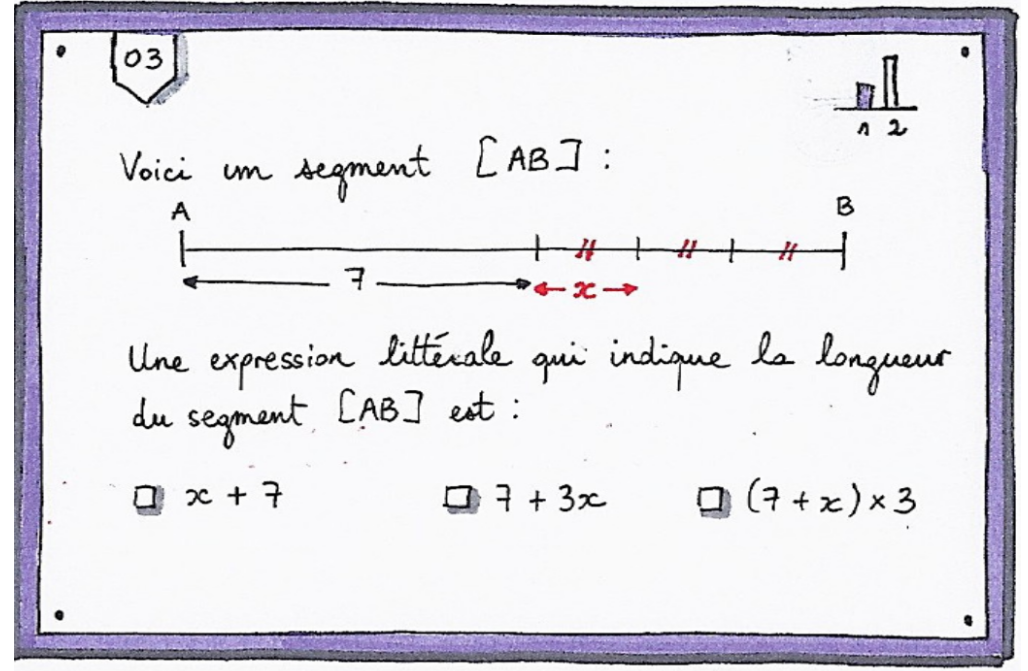
\includegraphics[width=\linewidth]{Images/CalculLitteral1.png}
            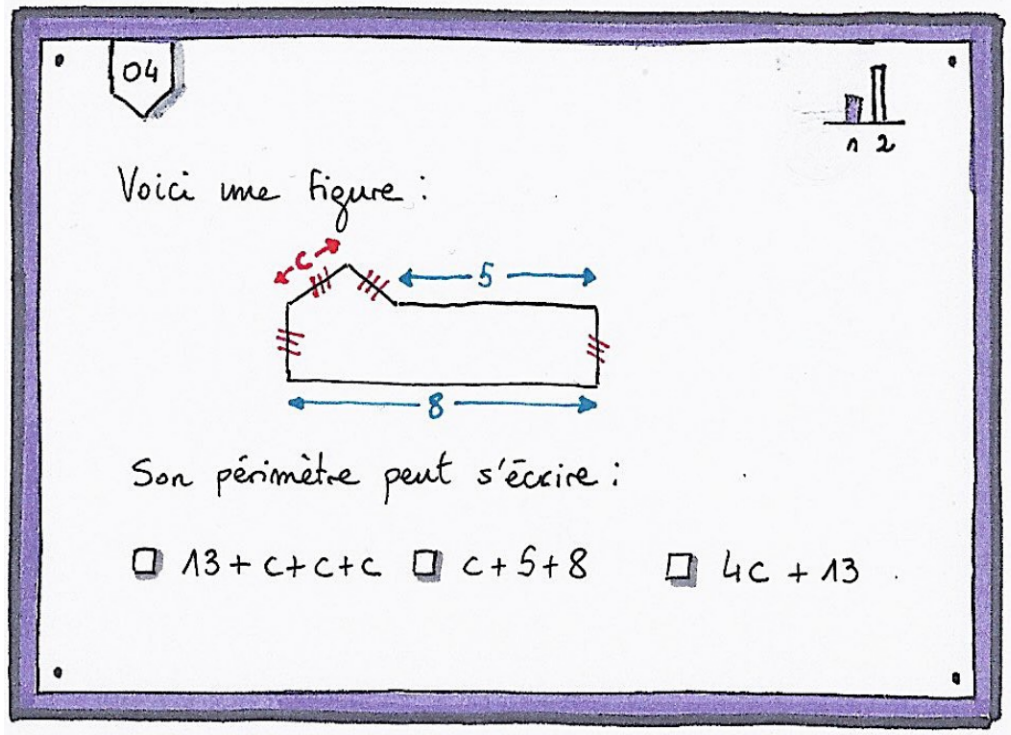
\includegraphics[width=\linewidth]{Images/CalculLitteral2.png}
        \end{exercice}

        \begin{exercice}
            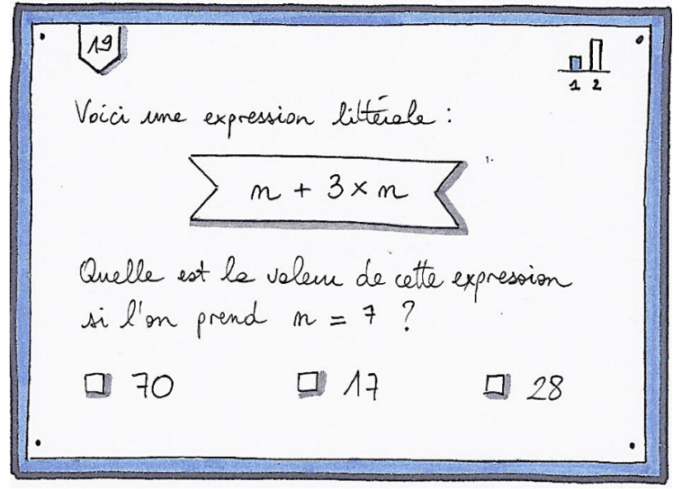
\includegraphics[width=0.95\linewidth]{Images/CalculLitteral3.png}
            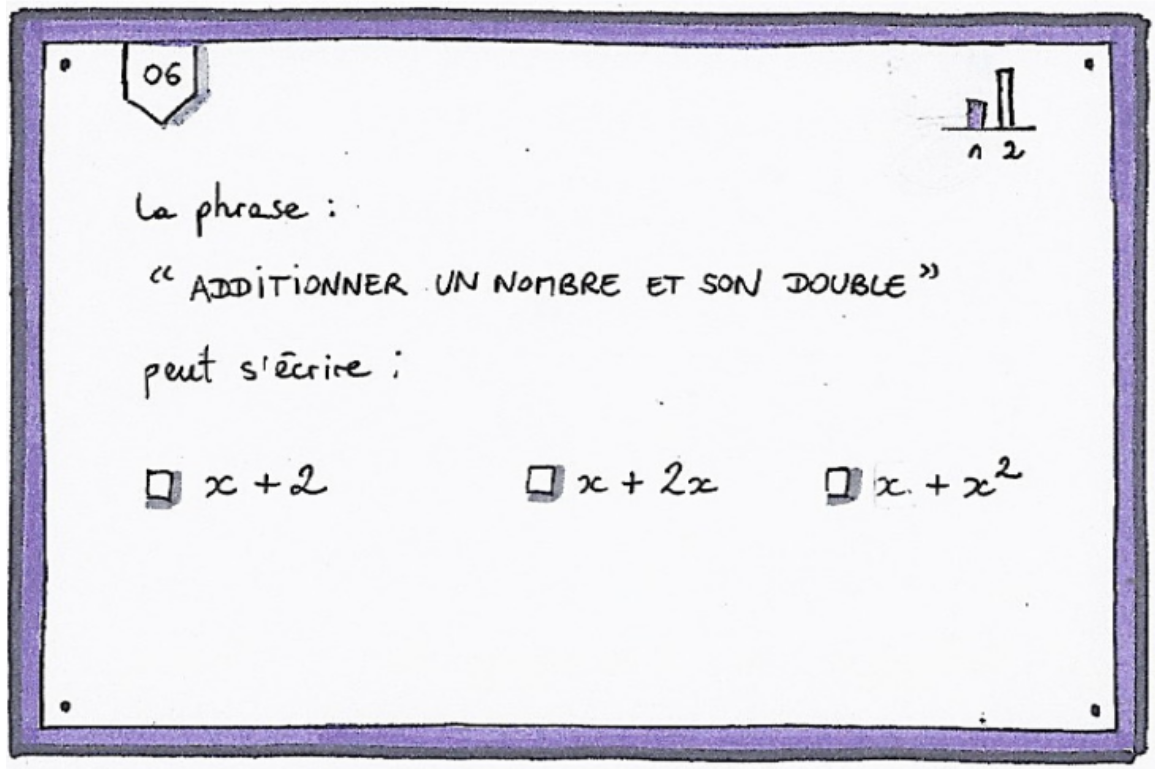
\includegraphics[width=0.95\linewidth]{Images/CalculLitteral4.png}
        \end{exercice}

        \begin{exercice}
            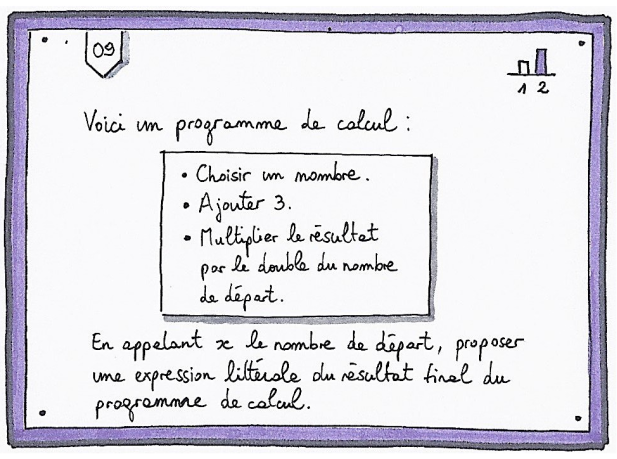
\includegraphics[width=0.95\linewidth]{Images/CalculLitteral5.png}
            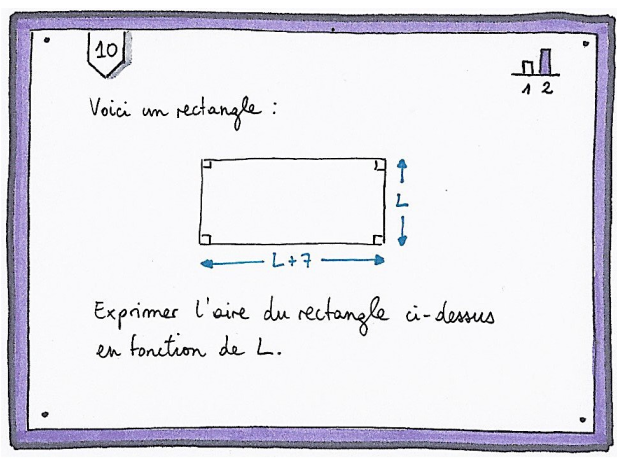
\includegraphics[width=0.95\linewidth]{Images/CalculLitteral6.png}
        \end{exercice}

        \begin{exercice}
            Réduire les exepressions suivantes.
            \begin{multicols}{2}
                \begin{enumerate}[label=\textbf{\alph*.}]
                    \item $6\times x$
                    \item $x \times 7$
                    \item $6\times a \times 2$
                    \item $a \times 3 \times b$
                    \item $4\times x \times 10\times y$
                    \item $2\times x \times 4 \times x$
                    \item $2x\times 5$
                    \item $3a \times 2a$
                    \item $-3 \times c \times 5$
                \end{enumerate}
            \end{multicols}
        \end{exercice}


        \begin{exercice}
            Réduire les exepressions suivantes.
            \begin{enumerate}[label=\textbf{\alph*.}]
                \item $6x + 2x$
                \item $6x + 2$
                \item $3a + 2 + 5a$
                \item $20y - 5 -2y$
                \item $5a + 10b - 2a + 3b$
                \item $3x -2 -2x + 10$
                \item $s + 9t + s - 10t$
                \item $5x^2 + 10x - 2x^2 + 4 - x + 1$
            \end{enumerate}
        \end{exercice}

        \columnbreak


        \begin{exercice}
            Recopier chaque expression, souligner les produits prioritaires, les réduire puis terminer en réduisant les sommes et différences.

            \vspace{.3cm}

            \textbf{Série 1}
            \begin{enumerate}[label=\textbf{\alph*.}]
                \item $6 + 2 \times x$
                \item $4 \times s + s \times 5 - 3$
                \item $-10 + 3 \times s + 2 \times 2$
                \item $y \times 5 + 3 - 2 \times y$
                \item $3 - 3 \times x + x \times 5$
                \item $4 \times 4 - 4 \times y - 4$
            \end{enumerate}
            \vspace{.3cm}
            \textbf{Série 2}
            \begin{enumerate}[label=\textbf{\alph*.}]
                \item $5 \times 3 + 2 \times d - 4$
                \item $5 + 3 \times e - 2 \times 3$
                \item $3 \times m - 3 \times m + 4$
                \item $8 \times h - 10 - h \times 7$
                \item $3 \times i + 4 \times 2 - i \times 2$
            \end{enumerate}
        \end{exercice}

        \begin{exercice}
            Recopier chaque expression, supprimer les parenthèses et réduire.\\
            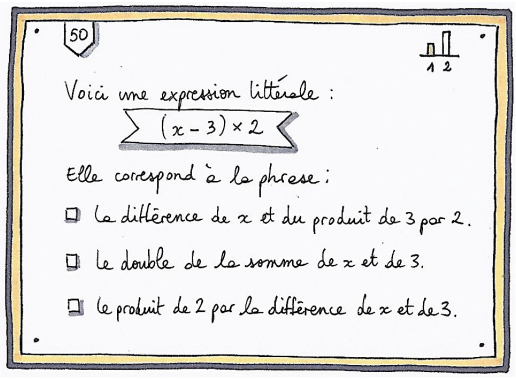
\includegraphics[width=\linewidth]{Images/CalculLitteral7.png}
        \end{exercice}

        \begin{exercice}
            Même consigne.\\
            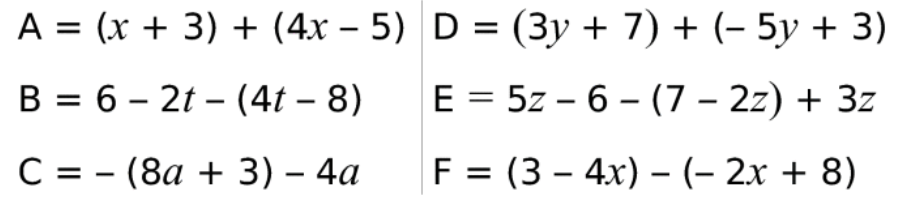
\includegraphics[width=\linewidth]{Images/CalculLitteral8.png}
        \end{exercice}

        \begin{exercice}
            Recopier chaque pyramide puis détailler sur ton cahier les calculs nécessaires pour compléter les cases vides en respectant les règles indiquées à droite.\\
            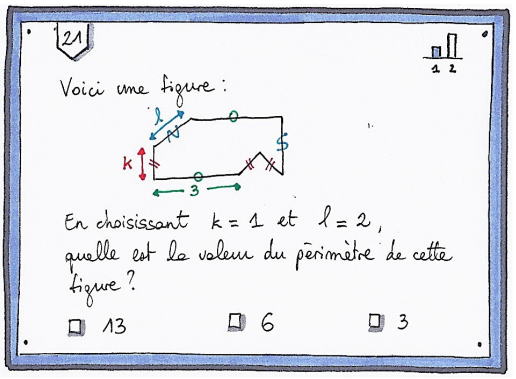
\includegraphics[width=\linewidth]{Images/CalculLitteral9.png}
        \end{exercice}

        \begin{exercice}
            Dans une expression, c’est la dernière opération effectuée (en respectant les priorités) qui permet de déterminer la nature de l’expression.
            \begin{itemize}
                \item $5 + x \times 2$ est une \emph{somme} car on termine par l’addition
                \item $(x - 4) \times 7$ est un \emph{produit} car on termine par la multiplication
            \end{itemize}
            Recopier chaque expression en mettant en couleur l’opération qui permet de déterminer sa nature.
            \begin{multicols}{2}
                \textbf{Série 1}
                \begin{enumerate}[label=\textbf{\alph*.}]
                    \item $ 5x + 3$
                    \item $ 7 - 2a $
                    \item $ (x + 1)(x- 1)$
                    \item $ \dfrac{x+y}{2}$
                \end{enumerate}
                \textbf{Série 2}
                \begin{enumerate}[label=\textbf{\alph*.}]
                    \item $ 2x + 6$
                    \item $ 2(x+3) $
                    \item $ \dfrac{2}{x^2 + y^2}$
                    \item $ (a+b)(a-b)+c$
                \end{enumerate}
            \end{multicols}
        \end{exercice}

        \begin{exercice}
            Recopier, développer et réduire.
            \begin{multicols}{2}
                \textbf{Série 1}
                \begin{enumerate}[label=\textbf{\alph*.}]
                    \item $ 3 \times \left( a+2 \right) $
                    \item $ 4 \left( 3+x \right) $
                    \item $ s \times \left( s+2 \right) $
                    \item $ 3u \left( u+4 \right) $
                    \item $ 5 \left( 4+a \right) $
                    \item $ s \left( 3+4s \right) $
                \end{enumerate}
                \textbf{Série 2}
                \begin{enumerate}[label=\textbf{\alph*.}]
                    \item $ 3 \times \left( 2+3a \right) $
                    \item $ 2s \left( 2+4s \right) $
                    \item $ \left( x+3 \right) \times 2 $
                    \item $ 5 \left( 2+x+y \right) $
                    \item $ x^2 \times \left( 3x+5 \right) $
                    \item $ a^2 \left( 3+a \right) $
                \end{enumerate}
            \end{multicols}
        \end{exercice}

        \begin{exercice}
            Recopier, développer et réduire.
            \begin{multicols}{2}
                \textbf{Série 1}
                \begin{enumerate}[label=\textbf{\alph*.}]
                    \item $ 2 \times \left( x-3 \right) $
                    \item $ 3 \times \left( 2s-1 \right) $
                    \item $ 2m \left( 5-4m \right) $
                    \item $ 5x \times \left( -2x+3 \right) $
                    \item $ 3 \times \left( -2-a \right) $
                    \item $ a \times \left( 2-2a \right) $
                \end{enumerate}
                \textbf{Série 2}
                \begin{enumerate}[label=\textbf{\alph*.}]
                    \item $ 2 \times \left( 3a+3 \right) $
                    \item $ 2x \times \left( x-2 \right) $
                    \item $ -4 \times \left( -3-x \right) $
                    \item $ -5x \times \left( 4x+3 \right) $
                    \item $ 5 \times \left( -4+4m \right) $
                    \item $ -a \times \left( -4a+2 \right) $
                \end{enumerate}
            \end{multicols}
        \end{exercice}

        \newpage

        \begin{exercice}
            \begin{center}
                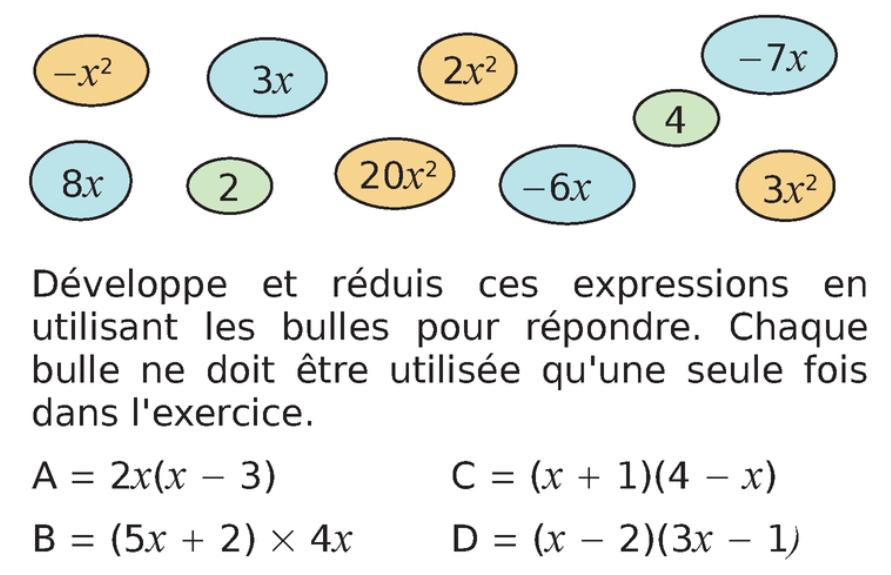
\includegraphics[width=\linewidth]{Images/CalculLitteral13.png}
            \end{center}
        \end{exercice}

        \begin{exercice}
            \begin{center}
                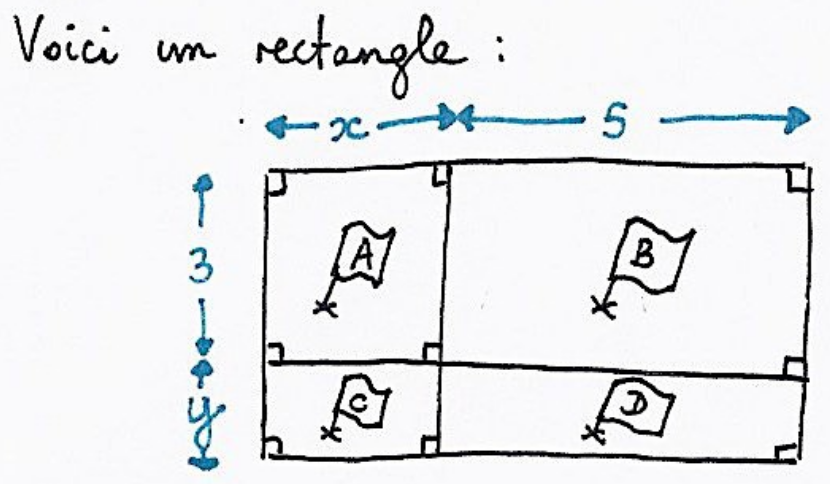
\includegraphics[width=\linewidth]{Images/Aire.png}
            \end{center}

            \begin{enumerate}
                \item Écris un produit qui permet de calculer l’aire du rectangle.
                \item Écris une somme de quatre termes qui est aussi égale à l’aire du rectangle.
            \end{enumerate}
        \end{exercice}
        \columnbreak

        \begin{exercice}
            Développer et réduire chaque expression.

                \textbf{Série 1}

                \begin{enumerate}[label=\textbf{\alph*.}]
                    \item $(x+5) \times (y+3)$
                    \item $(x + 4)\times (x+7)$
                    \item $(2x+5)(x+3)$
                    \item $(2a + 3)(5b + 7)$
                \end{enumerate}

                \textbf{Série 2}
                
                \begin{enumerate}[label=\textbf{\alph*.}]
                    \item $(7t + 3)(5 + 2t)$
                    \item $(y + 4)(y+4)$
                    \item $(2x+1)(3+x)$
                    \item $(x+2)(x+y+3)$
                \end{enumerate}
        \end{exercice}
        
        \begin{exercice}
            Développer et réduire.
                 \begin{enumerate}[label=\textbf{\alph*.}]
                    \item $(x-3)\times (x - 5)$
                    \item $(2y - 3)\times (-y+5)$
                    \item $(-x-3)(5x-7)$
                    \item $(x-2)(5x+3)$
                    \item $(-3+2z)(-4-5z)$
                    \item $(3t+5)(3t-5)$
                \end{enumerate}
        \end{exercice}
    \end{Maquette}

\end{multicols}

\end{document}
